\documentclass{article}
\usepackage{graphicx} % Required for inserting images
\usepackage{amsmath}
\usepackage{amssymb}
\usepackage{enumitem}
\usepackage{subfig}
\usepackage{tikz}

\begin{document}
\begin{center}
\textbf{
{\Large HKN ECE 120 Midterm 3 Worksheet}
} 
\end{center} 
\noindent\makebox[\linewidth]{\rule{\linewidth}{0.2pt}}

\section*{Serialized Design (Review)}
\subsection*{Problem 1}
Consider one bit-slice of a full adder.
\begin{enumerate}[label=\alph*.]
    \item How many bits need to be passed between each bit slice? What are they? \\
    \textbf{1 bit. We need to pass the carry bit between each bit slice.}
    \item If we wanted to serialize this design and add 1 bit at a time, how many D flip-flops would we need to store these signals? \\
    \textbf{1. We need 1 DFF for each signal we need to store.}
    \item Implement a serialized binary adder, adding 1 bit at a time.
    \begin{figure}[!h]
        \centering
        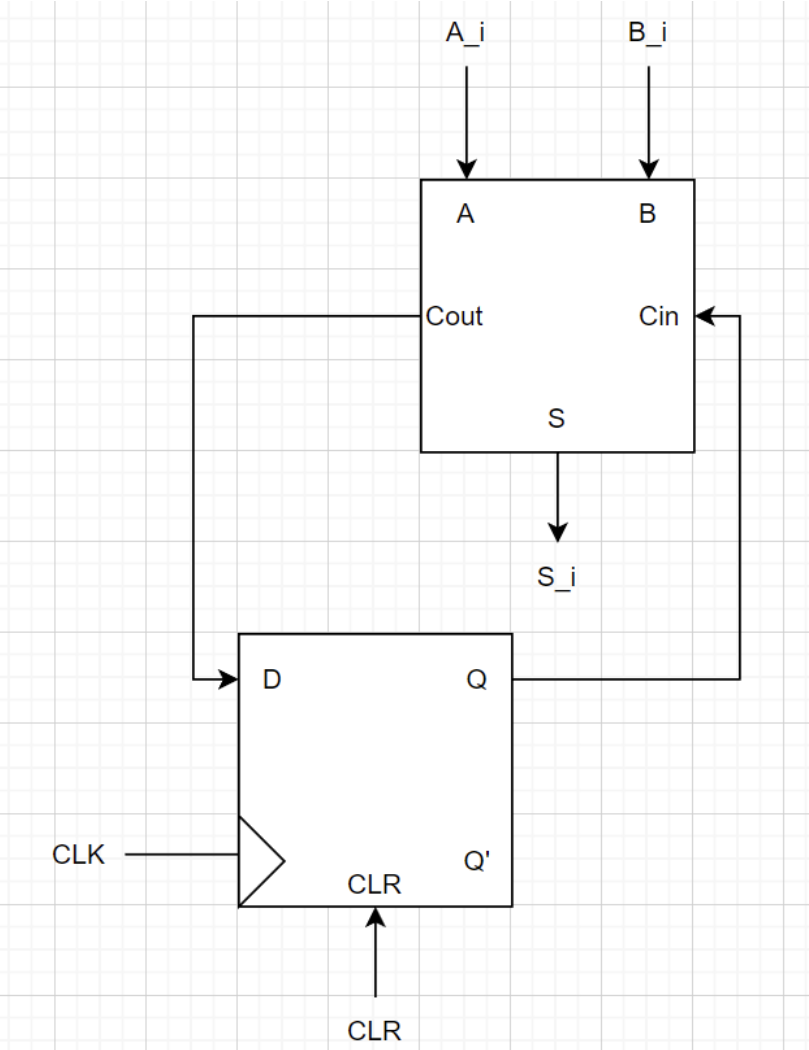
\includegraphics[width=0.5\textwidth]{figures/serial1c_solution.png}
    \end{figure}
    \\ \textbf{Note: the CLR (clear) signal is used when we want to clear the carry bit between adding different sets of numbers.}
    \item Assume we instead wanted to add 4 bits (1 hexadecimal) at a time. Would any signals be different?
    \\ \textbf{No, we still only need to pass one carry bit, the carry bit of the MSB, to the next clock cycle’s LSB.}
    \newpage
    \item Implement a serialized binary adder, adding 4 bits at a time.
    \begin{figure}[!h]
        \centering
        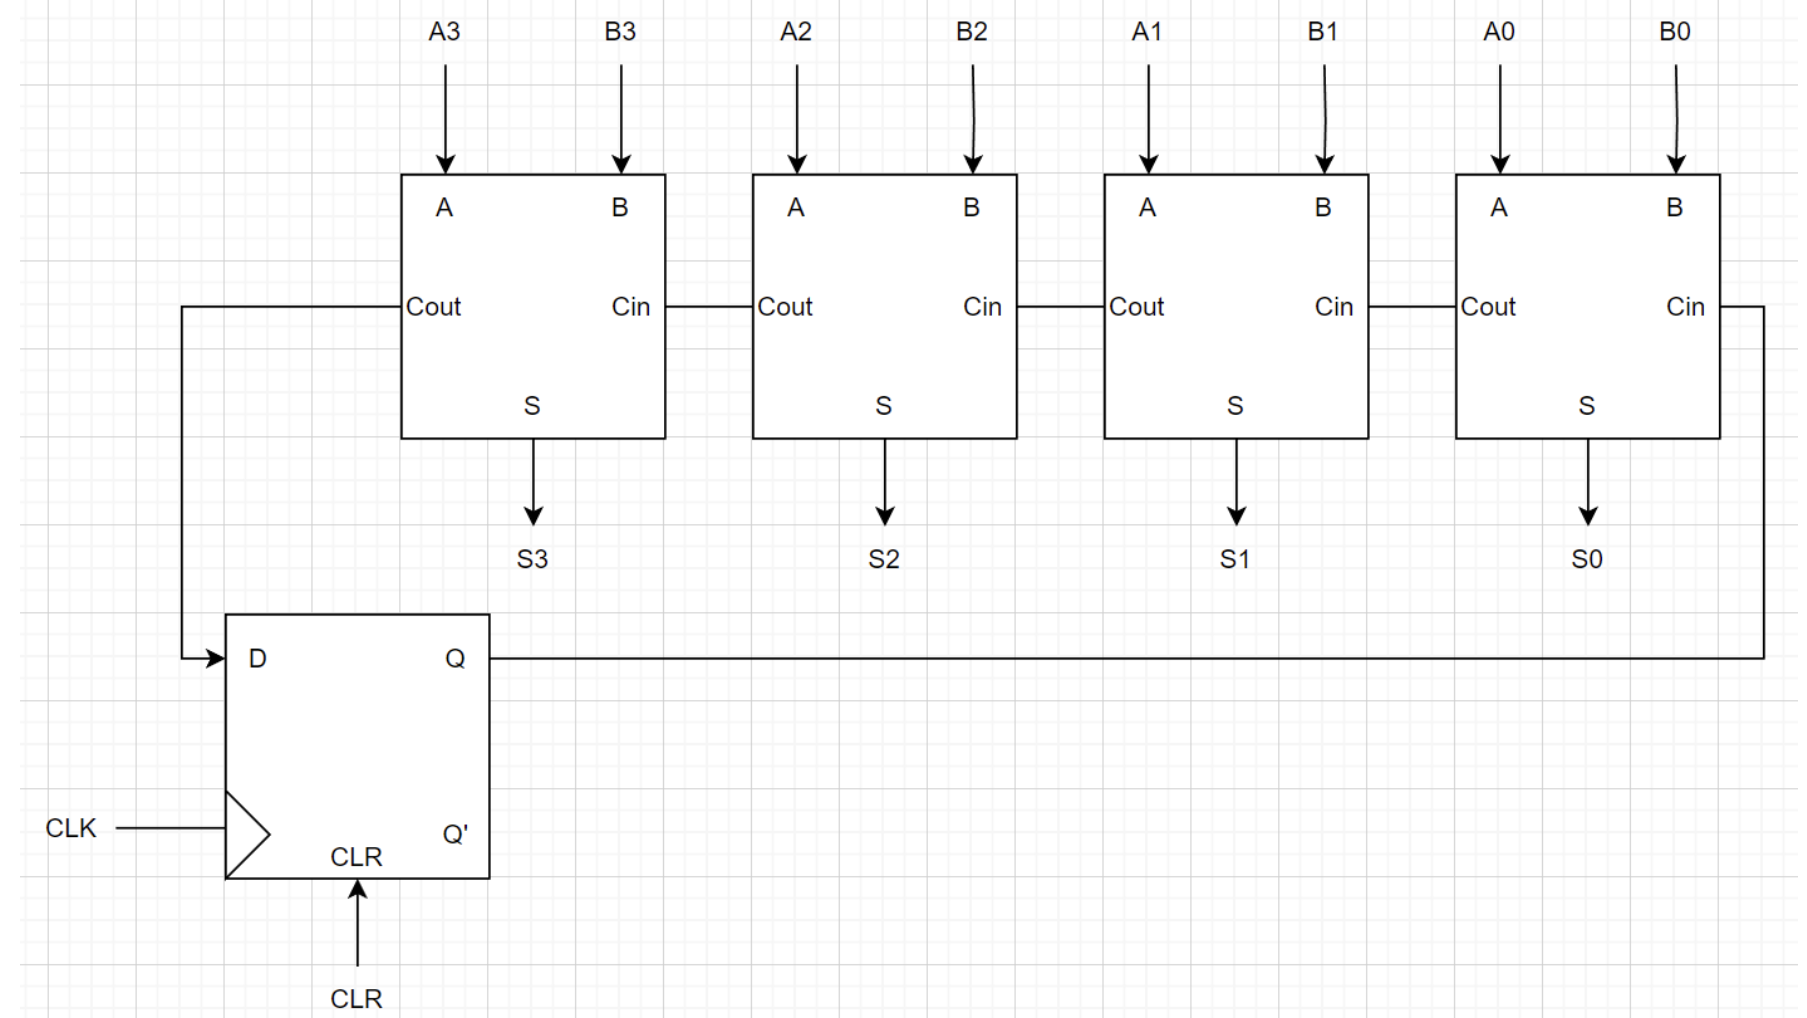
\includegraphics[width=1.1\textwidth]{figures/serial1e_solution.png}
    \end{figure}
\end{enumerate}


\subsection*{Problem 2}
Consider a serialized circuit that takes a sequence of bits, 1 bit at a time, and outputs the same sequence of bits but is delayed by 2 bits and inverted. For example, assuming inputs and outputs are taken at the start of each clock cycle, if the input is 100101101100, then the output is XX0110100100.
\begin{enumerate}[label=\alph*.]
    \item How many bits do we need to store between each clock cycle? \\
    \textbf{2 bits.}
    \item Implement this circuit using D flip-flops.
    \begin{figure}[!h]
        \centering
        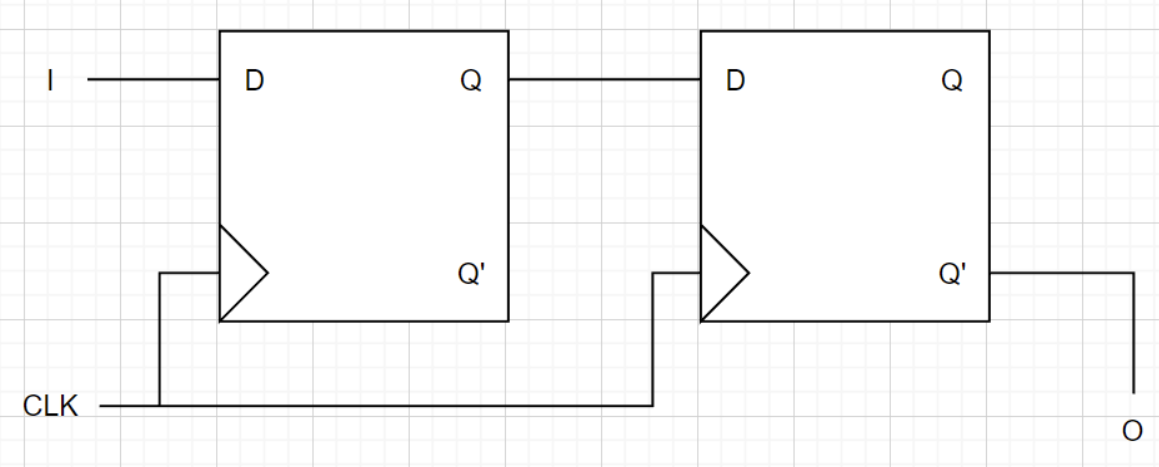
\includegraphics[width=1\textwidth]{figures/serial2b_solution.png}
    \end{figure}
    \item Can we also implement this circuit using a shift register? \\
    \textbf{Yes:}
    \begin{figure}[!h]
        \centering
        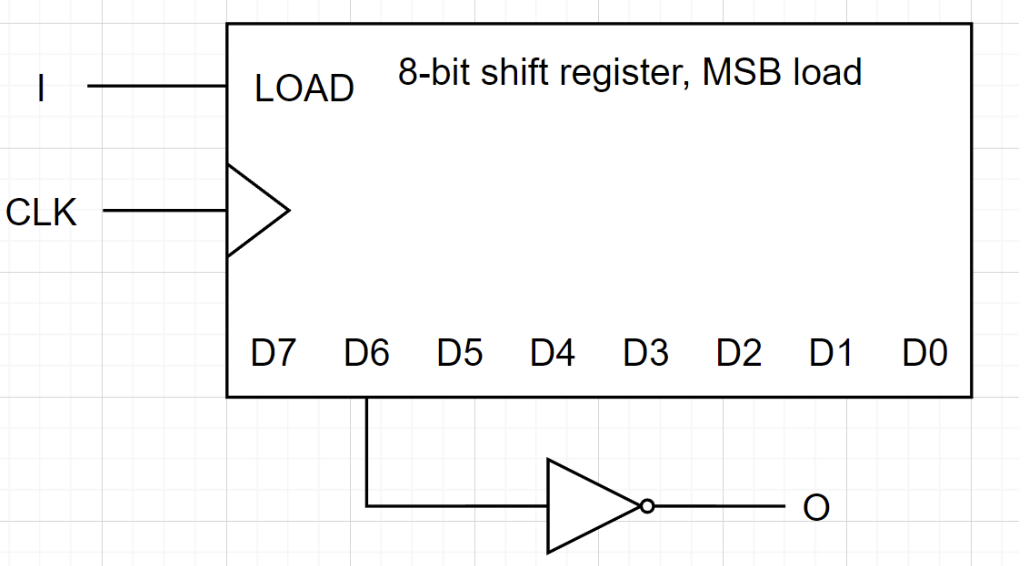
\includegraphics[width=0.8\textwidth]{figures/serial2c_solution.png}
    \end{figure}
\end{enumerate}


\subsection*{Problem 3}
In 50 words or less, what are the advantages and disadvantages of serialization over bit-slicing?\\ 
\\ \textbf{For larger sequences, serialized designs take much less area than bit-sliced designs. However, serialized designs are much slower, as they depend on the speed of a clock signal, while bit-sliced design is only dependent on gate delay. }


\newpage
\section*{Finite State Machines}
\subsection*{Problem 1}

Suppose we wanted to create a Moore FSM that has two outputs $Z$ and $O$. $Z$ is 1 if and only if the input contains three or more consecutive zeroes, and $O$ is 1 if and only if the input contains three or more consecutive ones.

\begin{enumerate}[label=\alph*.]
\item How many unique states do we need for this finite state machine? How many bits do we need to represent all states?
\textbf{6 states. For both 0s and 1s, we want to keep track of how many we have seen consecutively. We have one state for seeing one, two, and three or more for both 0 and 1, so 6 states. We can represent it with 3 bits, allowing for up to 8 states. }
\item Draw a state diagram for this FSM, showing all states used.
\textbf{This is one possible enumeration.}
\begin{figure}[!h]
    \centering
    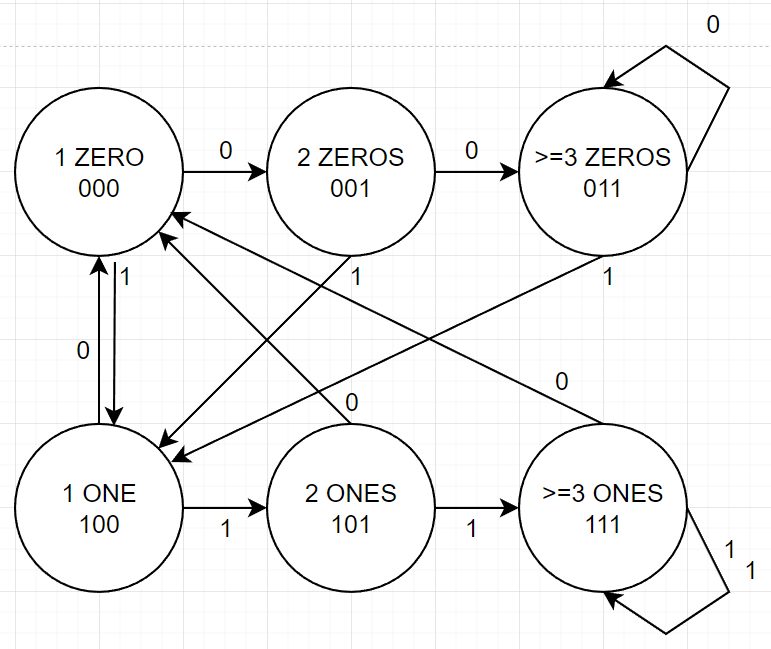
\includegraphics[width=0.8\textwidth]{figures/fsm1b-solution.png}
\end{figure}
\item Create a truth table for this FSM. For unused states, write $X$.
\begin{table}[!h]
\begin{tabular}{|l|l|l|l|l|l|l|}
\hline
S\_2 & S\_1 & S\_0 & A (input) & $S\_2^+$ & $S\_1^+$ & $S\_0^+$ \\ \hline
0    & 0    & 0    & 0         & 0                       & 0                       & 1                       \\ \hline
0    & 0    & 0    & 1         & 1                       & 0                       & 0                       \\ \hline
0    & 0    & 1    & 0         & 0                       & 1                       & 1                       \\ \hline
0    & 0    & 1    & 1         & 1                       & 0                       & 0                       \\ \hline
0    & 1    & 0    & 0         & X                       & X                       & X                       \\ \hline
0    & 1    & 0    & 1         & X                       & X                       & X                       \\ \hline
0    & 1    & 1    & 0         & 0                       & 1                       & 1                       \\ \hline
0    & 1    & 1    & 1         & 1                       & 0                       & 0                       \\ \hline
1    & 0    & 0    & 0         & 0                       & 0                       & 0                       \\ \hline
1    & 0    & 0    & 1         & 1                       & 0                       & 1                       \\ \hline
1    & 0    & 1    & 0         & 0                       & 0                       & 0                       \\ \hline
1    & 0    & 1    & 1         & 1                       & 1                       & 1                       \\ \hline
1    & 1    & 0    & 0         & X                       & X                       & X                       \\ \hline
1    & 1    & 0    & 1         & X                       & X                       & X                       \\ \hline
1    & 1    & 1    & 0         & 0                       & 0                       & 0                       \\ \hline
1    & 1    & 1    & 1         & 1                       & 1                       & 1                       \\ \hline
\end{tabular}
\end{table}
\newpage

\item Use K-maps or another method to derive next-state expressions for this FSM. \\
\textbf{
$S_2^+ = A$\\
$S_1^+ = S_2'S_0A'+S_2S_0A$ \\
$S_0^+ = S_2'A' + S_2A$
}
\\ \\
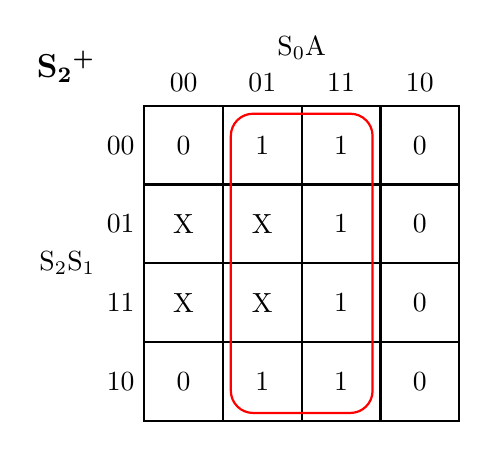
\begin{tikzpicture}
    % Draw grid for Karnaugh map
    \draw[thick] (0, 0) rectangle (4, 4);
    \foreach \x in {1, 2, 3} {
        \draw[thick] (\x, 0) -- (\x, 4);
        \draw[thick] (0, \x) -- (4, \x);
    }

    % Labels for columns
    \node at (0.5, 4.3) {00};
    \node at (1.5, 4.3) {01};
    \node at (2.5, 4.3) {11};
    \node at (3.5, 4.3) {10};

    % Labels for rows
    \node at (-0.3, 3.5) {00};
    \node at (-0.3, 2.5) {01};
    \node at (-0.3, 1.5) {11};
    \node at (-0.3, 0.5) {10};

    % Example entries in cells (you can replace with your values)
    \node at (0.5, 3.5) {0};
    \node at (1.5, 3.5) {1};
    \node at (2.5, 3.5) {1};
    \node at (3.5, 3.5) {0};

    \node at (0.5, 2.5) {X};
    \node at (1.5, 2.5) {X};
    \node at (2.5, 2.5) {1};
    \node at (3.5, 2.5) {0};

    \node at (0.5, 1.5) {X};
    \node at (1.5, 1.5) {X};
    \node at (2.5, 1.5) {1};
    \node at (3.5, 1.5) {0};

    \node at (0.5, 0.5) {0};
    \node at (1.5, 0.5) {1};
    \node at (2.5, 0.5) {1};
    \node at (3.5, 0.5) {0};

    % Label axes (optional)
    \node[anchor=east] at (-0.5, 2){S\textsubscript{2}S\textsubscript{1}};
    \node[anchor=north] at (2, 5) {S\textsubscript{0}A};
    \node[anchor=east] at (-.5,4.5){\large\textbf{S\textsubscript{2}\textsuperscript{+}}};
    % Loops (grouping cells)
    % Group of two horizontally
    \draw[rounded corners=8pt, red, thick] (1.1, 3.9) rectangle (2.9, 0.1);
    % Group of four

\end{tikzpicture}
\\ \\ \\ \\
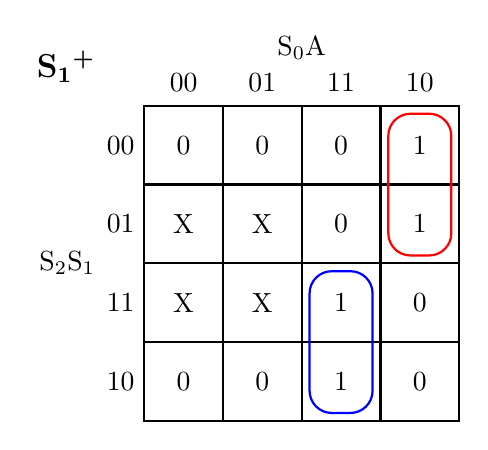
\begin{tikzpicture}
    % Draw grid for Karnaugh map
    \draw[thick] (0, 0) rectangle (4, 4);
    \foreach \x in {1, 2, 3} {
        \draw[thick] (\x, 0) -- (\x, 4);
        \draw[thick] (0, \x) -- (4, \x);
    }

    % Labels for columns
    \node at (0.5, 4.3) {00};
    \node at (1.5, 4.3) {01};
    \node at (2.5, 4.3) {11};
    \node at (3.5, 4.3) {10};

    % Labels for rows
    \node at (-0.3, 3.5) {00};
    \node at (-0.3, 2.5) {01};
    \node at (-0.3, 1.5) {11};
    \node at (-0.3, 0.5) {10};

    % Example entries in cells (you can replace with your values)
    \node at (0.5, 3.5) {0};
    \node at (1.5, 3.5) {0};
    \node at (2.5, 3.5) {0};
    \node at (3.5, 3.5) {1};

    \node at (0.5, 2.5) {X};
    \node at (1.5, 2.5) {X};
    \node at (2.5, 2.5) {0};
    \node at (3.5, 2.5) {1};

    \node at (0.5, 1.5) {X};
    \node at (1.5, 1.5) {X};
    \node at (2.5, 1.5) {1};
    \node at (3.5, 1.5) {0};

    \node at (0.5, 0.5) {0};
    \node at (1.5, 0.5) {0};
    \node at (2.5, 0.5) {1};
    \node at (3.5, 0.5) {0};

    % Label axes (optional)
    \node[anchor=east] at (-0.5, 2){S\textsubscript{2}S\textsubscript{1}};
    \node[anchor=north] at (2, 5) {S\textsubscript{0}A};
    \node[anchor=east] at (-.5,4.5){\large\textbf{S\textsubscript{1}\textsuperscript{+}}};
    % Loops (grouping cells)
    % Group of two horizontally
    \draw[rounded corners=8pt, red, thick] (3.1, 3.9) rectangle (3.9, 2.1);
    % Group of four
    \draw[rounded corners=8pt, blue, thick] (2.1, 1.9) rectangle (2.9, 0.1);

\end{tikzpicture}
\\ \\ \\ \\
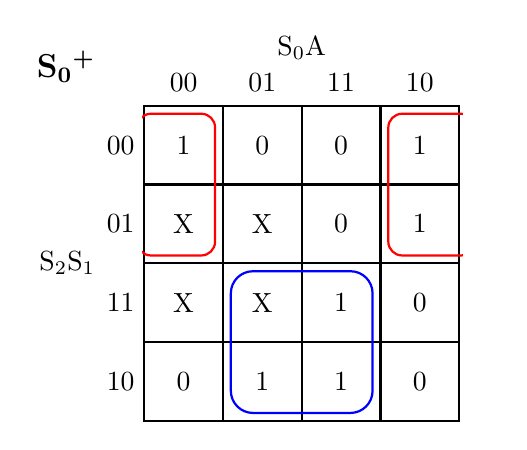
\begin{tikzpicture}
    % Draw grid for Karnaugh map
    \draw[thick] (0, 0) rectangle (4, 4);
    \foreach \x in {1, 2, 3} {
        \draw[thick] (\x, 0) -- (\x, 4);
        \draw[thick] (0, \x) -- (4, \x);
    }

    % Labels for columns
    \node at (0.5, 4.3) {00};
    \node at (1.5, 4.3) {01};
    \node at (2.5, 4.3) {11};
    \node at (3.5, 4.3) {10};

    % Labels for rows
    \node at (-0.3, 3.5) {00};
    \node at (-0.3, 2.5) {01};
    \node at (-0.3, 1.5) {11};
    \node at (-0.3, 0.5) {10};

    % Example entries in cells (you can replace with your values)
    \node at (0.5, 3.5) {1};
    \node at (1.5, 3.5) {0};
    \node at (2.5, 3.5) {0};
    \node at (3.5, 3.5) {1};

    \node at (0.5, 2.5) {X};
    \node at (1.5, 2.5) {X};
    \node at (2.5, 2.5) {0};
    \node at (3.5, 2.5) {1};

    \node at (0.5, 1.5) {X};
    \node at (1.5, 1.5) {X};
    \node at (2.5, 1.5) {1};
    \node at (3.5, 1.5) {0};

    \node at (0.5, 0.5) {0};
    \node at (1.5, 0.5) {1};
    \node at (2.5, 0.5) {1};
    \node at (3.5, 0.5) {0};

    % Label axes (optional)
    \node[anchor=east] at (-0.5, 2){S\textsubscript{2}S\textsubscript{1}};
    \node[anchor=north] at (2, 5) {S\textsubscript{0}A};
    \node[anchor=east] at (-.5,4.5){\large\textbf{S\textsubscript{0}\textsuperscript{+}}};
    % Loops (grouping cells)
    % Group of two horizontally

    % Group of four
    \draw[rounded corners=8pt, blue, thick] (1.1, 1.9) rectangle (2.9, 0.1);
    \draw[rounded corners=5pt, red, thick] (3.1, 3.9) rectangle (4.2, 2.1);
    \draw[rounded corners=5pt, red, thick] (-.09, 3.9) rectangle (0.9, 2.1);
    \fill[white](-.12,3.9) rectangle (-.03, 2.1);
    \fill[white] (4.05, 4) rectangle (4.5, 2);

\end{tikzpicture}
\item Implement this FSM using D flip-flops.
\begin{figure}[!h]
    \centering
    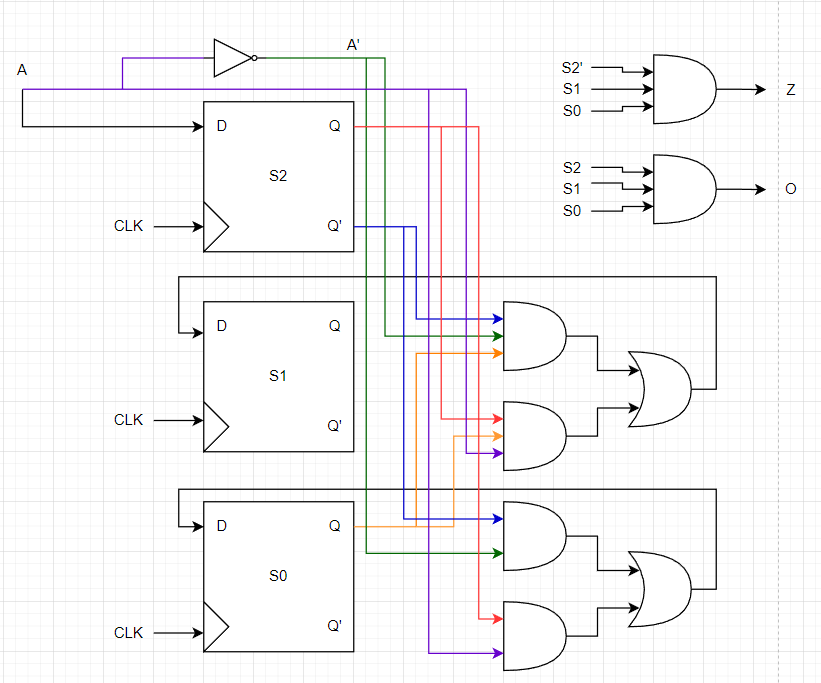
\includegraphics[width=0.8\textwidth]{figures/fsm1e-solution.png}
\end{figure}
\end{enumerate}

\newpage
\subsection*{Problem 2}

Suppose we wanted to create a Mealy FSM that represents an elevator in a building with 6 floors, 1 through 6. It takes two clock cycles for the elevator to move between floors. The input is a 3-bit unsigned integer $I_2I_1I_0$ and the output is a single bit $F$ that is 1 when the elevator has reached the correct floor and 0 when it has not. You may assume that the input is always between 1 and 6 (inclusive).

\begin{enumerate}[label=\alph*.]
\item How many unique states do we need for this finite state machine? How many bits do we need to represent all states?
\textbf{We need a state for each of the floors and another state for moving between floors. Since there are 6 floors, we need 6 floors, plus 5 in-between states, so we need 11 states. We can represent this with 4 bits, allowing for up to 16 states.}
\newpage
\item Draw a state diagram for this FSM, showing all states used. You may also use comparisons ($=, <, >$). (Hint: it might be helpful to enumerate the states in a way that preserves the 3-bit floor) \\
\textbf{This is probably the easiest enumeration, but others are possible.}
\begin{figure}[!h]
    \centering
    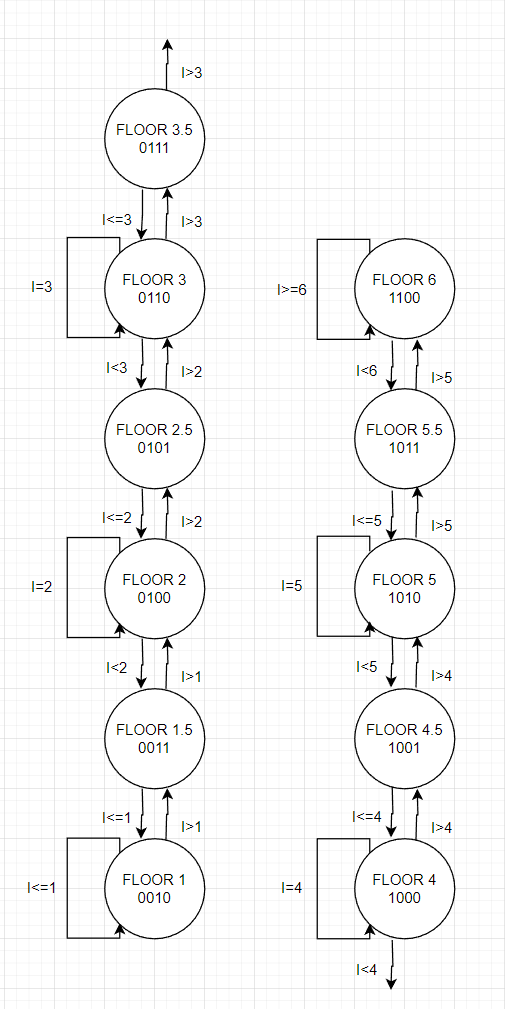
\includegraphics[width=0.5\textwidth]{figures/fsm2b-solution.png}
\end{figure}
\newpage
\item Create a truth table for this FSM, defining new intermediate variables for your comparisons. For unused states, write $X$.\\
$E = (I = S_3S_2S_1)$ \\
$L = (I < S_3S_2S_1)$ \\
$G = (I > S_3S_2S_1)$ \\
\begin{table}[!h]
\begin{tabular}{|l|l|l|l|l|}
\hline
L & E & G & $S_0$ & $S^+$ \\ \hline
0 & 0 & 0 & 0    & XXXX                 \\ \hline
0 & 0 & 0 & 1    & XXXX                 \\ \hline
0 & 0 & 1 & 0    & S + 1                \\ \hline
0 & 0 & 1 & 1    & S + 1                \\ \hline
0 & 1 & 0 & 0    & S                    \\ \hline
0 & 1 & 0 & 1    & S - 1                \\ \hline
0 & 1 & 1 & 0    & XXXX                 \\ \hline
0 & 1 & 1 & 1    & XXXX                 \\ \hline
1 & 0 & 0 & 0    & S - 1                \\ \hline
1 & 0 & 0 & 1    & S - 1                \\ \hline
1 & 0 & 1 & 0    & XXXX                 \\ \hline
1 & 0 & 1 & 1    & XXXX                 \\ \hline
1 & 1 & 0 & 0    & XXXX                 \\ \hline
1 & 1 & 0 & 1    & XXXX                 \\ \hline
1 & 1 & 1 & 0    & XXXX                 \\ \hline
1 & 1 & 1 & 1    & XXXX                 \\ \hline
\end{tabular}
\end{table}
\item Use K-maps or another method to derive next-state expressions for this FSM. \\
$S^+ = (S + 1)G + (S - 1)(L + ES_0) + (S)(ES_0')$
\\ \\
% kmap for problem 2 fsms
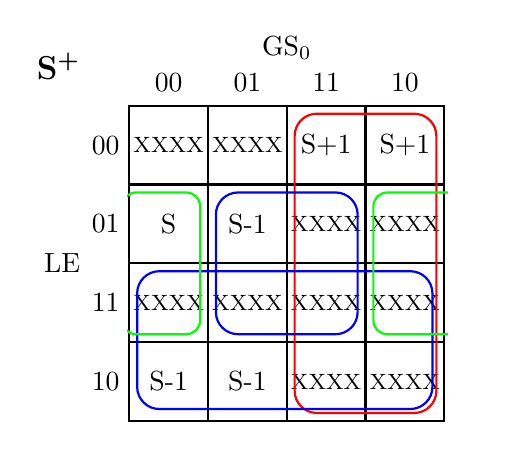
\begin{tikzpicture}
    % Draw grid for Karnaugh map
    \draw[thick] (0, 0) rectangle (4, 4);
    \foreach \x in {1, 2, 3} {
        \draw[thick] (\x, 0) -- (\x, 4);
        \draw[thick] (0, \x) -- (4, \x);
    }

    % Labels for columns
    \node at (0.5, 4.3) {00};
    \node at (1.5, 4.3) {01};
    \node at (2.5, 4.3) {11};
    \node at (3.5, 4.3) {10};

    % Labels for rows
    \node at (-0.3, 3.5) {00};
    \node at (-0.3, 2.5) {01};
    \node at (-0.3, 1.5) {11};
    \node at (-0.3, 0.5) {10};

    % Example entries in cells (you can replace with your values)
    \node at (0.5, 3.5) {\footnotesize{XXXX}};
    \node at (1.5, 3.5) {\footnotesize{XXXX}};
    \node at (2.5, 3.5) {S+1};
    \node at (3.5, 3.5) {S+1};

    \node at (0.5, 2.5) {S};
    \node at (1.5, 2.5) {S-1};
    \node at (2.5, 2.5) {\footnotesize{XXXX}};
    \node at (3.5, 2.5) {\footnotesize{XXXX}};

    \node at (0.5, 1.5) {\footnotesize{XXXX}};
    \node at (1.5, 1.5) {\footnotesize{XXXX}};
    \node at (2.5, 1.5) {\footnotesize{XXXX}};
    \node at (3.5, 1.5) {\footnotesize{XXXX}};

    \node at (0.5, 0.5) {S-1};
    \node at (1.5, 0.5) {S-1};
    \node at (2.5, 0.5) {\footnotesize{XXXX}};
    \node at (3.5, 0.5) {\footnotesize{XXXX}};

    % Label axes (optional)
    \node[anchor=east] at (-0.5, 2){LE};
    \node[anchor=north] at (2, 5) {GS\textsubscript{0}};
    \node[anchor=east] at (-.5,4.5){\large\textbf{S\textsuperscript{+}}};
    % Loops (grouping cells)
    % Group of two horizontally
    \draw[rounded corners=8pt, red, thick] (2.1, 3.9) rectangle (3.9, 0.1);
    % Group of four
    \draw[rounded corners=8pt, blue, thick] (0.1, 1.9) rectangle (3.85, 0.15);
    \draw[rounded corners=8pt, blue, thick] (1.1, 2.9) rectangle (2.9, 1.1);
    %wraparound
    \draw[rounded corners=5pt, green, thick] (3.1, 2.9) rectangle (4.2, 1.1);
    \draw[rounded corners=5pt, green, thick] (-.09, 2.9) rectangle (0.9, 1.1);
    \fill[white](-.12,3.9) rectangle (-.03, 1.1);
    \fill[white] (4.05, 4) rectangle (4.5, 1);


\end{tikzpicture}
\newpage
\item Implement this FSM using D flip-flops and a 3-bit digital comparator, with outputs for $A > B$, $A = B$, and $A < B$. Feel free to use adders, MUXes, buses, or any other component covered earlier in the course.
\begin{figure}[!h]
    \centering
    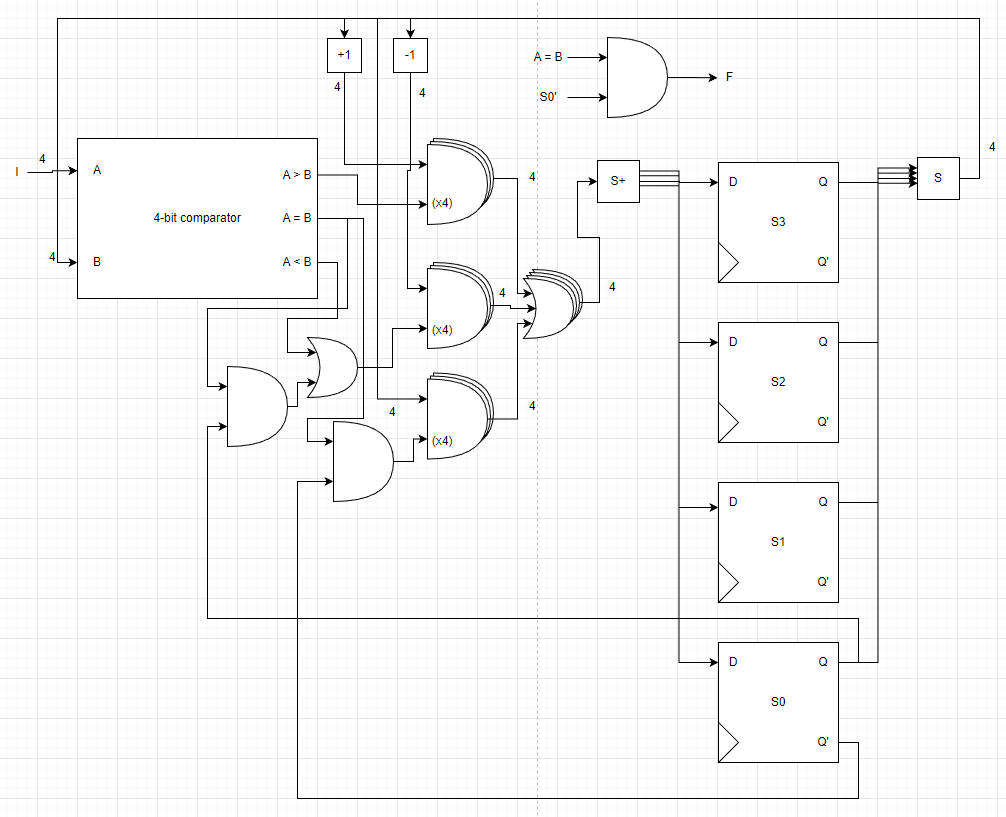
\includegraphics[width=1\textwidth]{figures/fsm2e-solution.png}
\end{figure}
\end{enumerate}

\newpage
\subsection*{Problem 3}
Taken from HDLBits "Design a Moore FSM"\\
\begin{figure}[!h]
    \centering
    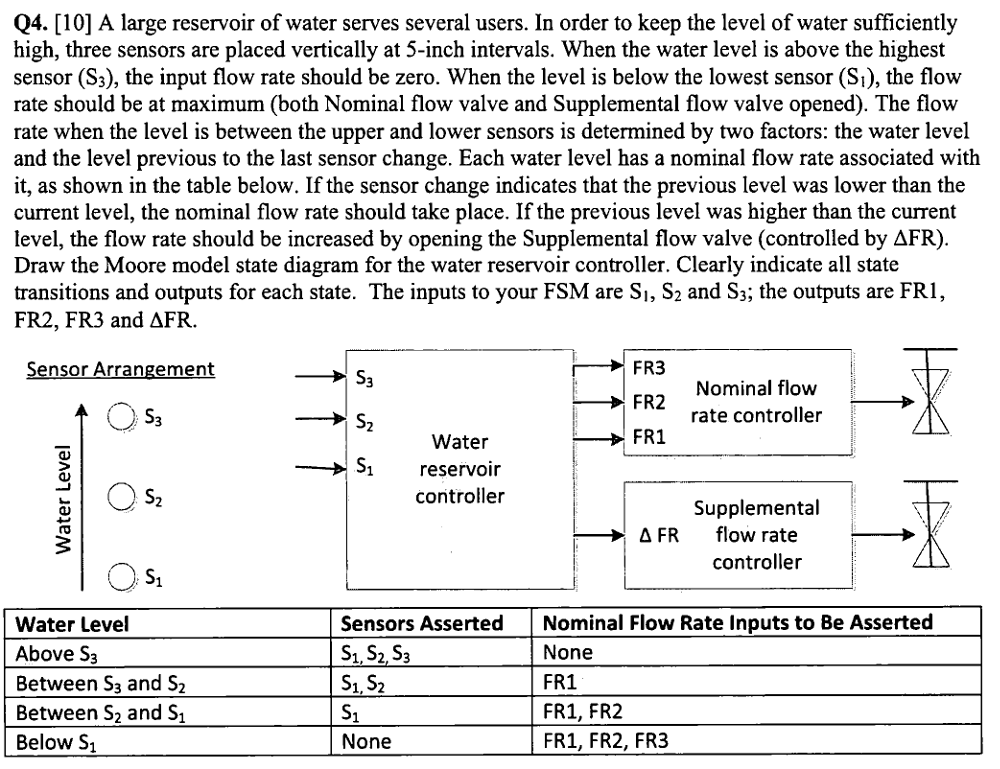
\includegraphics[width=0.7\textwidth]{figures/fsm_q3.png}
\end{figure}
\begin{figure}[!h]
    \centering
    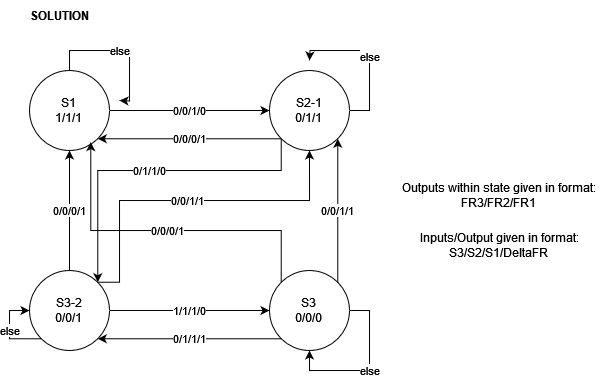
\includegraphics[width=1\textwidth]{figures/fsm_q3-solution.png}
\end{figure}



\newpage
\section*{Memory}
\subsection*{Problem 1}

\begin{enumerate}[label=\alph*.]
\item What is memory addressability? What is the difference between memory addressability and a memory address? \\
\textbf{The number of addresses, or address space, is the number of memory locations in a memory module. The addressibility is the number of bits of memory that can be accessed at once at a memory location, corresponding to a memory address.}
\item What is the purpose of the chip select signal in a RAM block? \\
\textbf{The chip select signal allows for our control logic to control which memory modules are enabled, allowing us to share connections between memory modules.}
\item What is the purpose of the write enable signal in a RAM block? \\
\textbf{The write enable signal allows us to select between reading and writing on a memory module.}
\item Describe the process to read from a RAM block. Detail the signal values: \\
\textbf{Chip select should be set to high (active), and write enable should be set to low (inactive). Note that some modules show $\overline{WE}$, which indicate active low, so write enable should be set to high in that case.}
\item Describe the process to write to a RAM block. Detail the signal values: \\
\textbf{Chip select should be set to high (active), and write enable should be set to high (active). Again, if write enable is active low, it should be set to low. }

\end{enumerate}
\newpage
\subsection*{Problem 2}
\begin{figure}[!h]
    \centering
    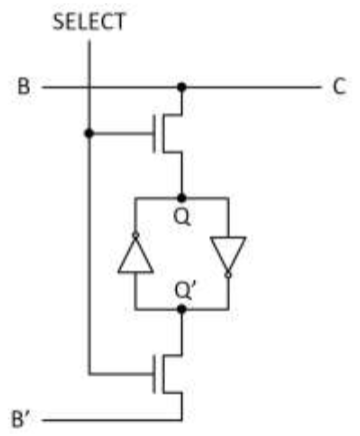
\includegraphics[width=0.3\textwidth]{figures/memory_q2.png}
\end{figure}

\begin{enumerate}[label=\alph*.]
\item What should we apply to Select, B and B’ in order to read the value Q to C? \\
\textbf{SELECT = 1, B = High-Z, B' = High-Z}
\item What should we apply to Select, B and B’ in order to hold a value Q? \\
\textbf{SELECT = 0, B = High-Z, B' = High-Z}
\item What should we apply to Select, B and B’ in order to write a 0 to Q? \\
\textbf{SELECT = 1, B = 0, B' = 1}
\item What should we apply to Select, B and B’ in order to write a 1 to Q?
\textbf{SELECT = 1, B = 1, B' = 0}
\end{enumerate}

\newpage
\subsection*{Problem 3}
\begin{figure}[!h]
    \centering
    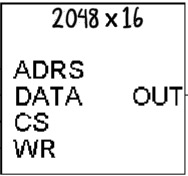
\includegraphics[width=0.3\textwidth]{figures/memory_q1.jpg}
\end{figure}
For each of the combinations below, select and draw those that can be used to build a 2048 x 12 RAM using only the parts given. If not possible, explain why. Assume that logic 0 and 1 signals are available and that the chip select and write enable are active-high.

\begin{enumerate}[label=\alph*.]
\item Two 1024 x 6 RAMs and one 4:1 multiplexer \\
\textbf{Not possible. The largest we can build is a 2048 x 6 or 1024 x 12 RAM.}
\item Four 512 x 12 RAMs and a 2:4 priority encoder
\begin{figure}[!h]
    \centering
    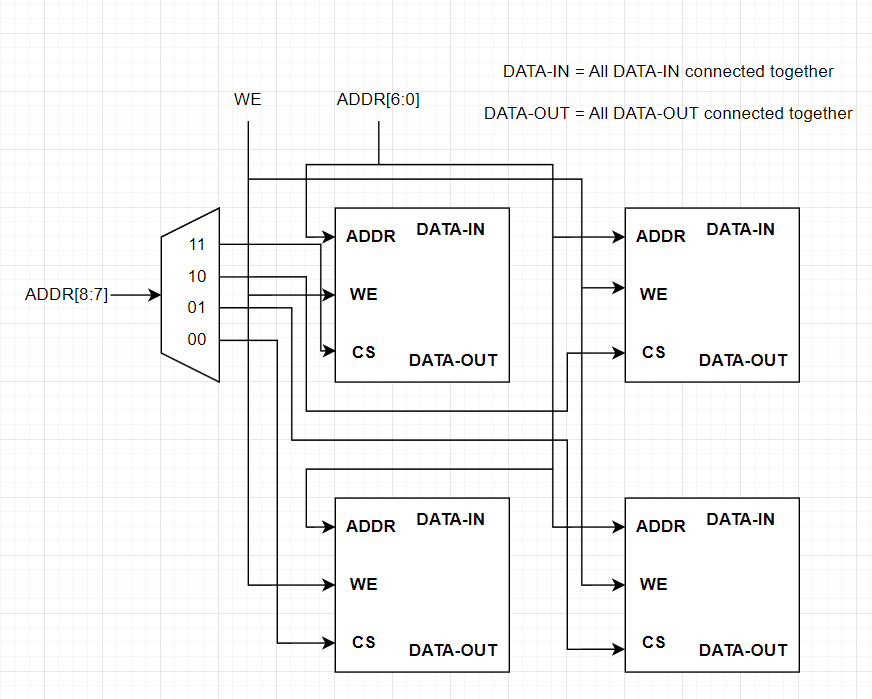
\includegraphics[width=0.3\textwidth]{figures/memory3b-solution.png}
\end{figure}
\item Two 2048 x 6 RAMs	
\begin{figure}[!h]
    \centering
    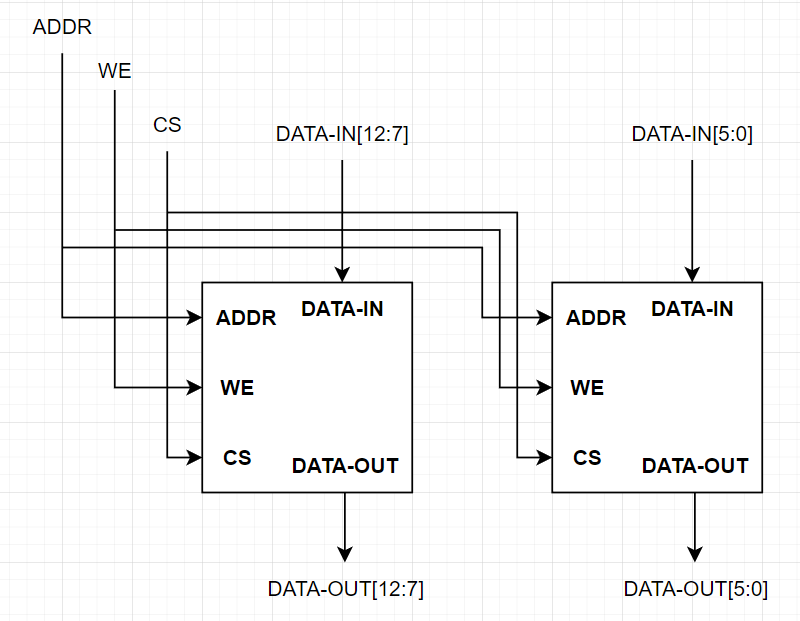
\includegraphics[width=0.3\textwidth]{figures/memory3c-solution.png}
\end{figure}
\item Four 512 x 3 RAMs and two 4:1 multiplexers \\
\textbf{Not possible. The largest we can build is a 2048 x 3 or 512 x 12 RAM.}
\end{enumerate}


\newpage
\section*{LC-3 ISA}
\subsection*{Problem 1}
Review Questions. Answer for the LC-3 ISA.
\begin{enumerate}[label=\alph*.]
\item How many bits are used to address memory? What is the memory address space? \\
\textbf{The LC-3 has 16 bit memory addresses. Its address space is $2^{16}$, or 65536 locations.}
\item How many bits of data are stored at each memory space/what is the memory addressibility? \\
\textbf{The LC-3 has a 16 bit memory bus. Its memory addressibility is 16 bits. }
\item What is the bus width? \\
\textbf{The LC-3 has a system bus that is also 16 bits wide. By making all bus sizes be the same, we don't have to do conversions between different sized buses.}
\item How many registers are in the register file? How wide are they? \\
\textbf{8 registers, R0 through R7. They are each 16 bits wide.}
\item How many other registers are there? How wide are they? \\
\textbf{At least 5. We have the Program Counter (PC), the Instruction Register (IR), the Memory Address Register (MAR), the Memory Data Register (MDR), control codes (NZP), and more registers for I/O (not taught in ECE 120).}
\item How do we control which signals are sent to the system bus? \\
\textbf{Tri-state buffers are added wherever there is a connection into the system bus, allowing for control logic to ensure only one is enabled at any one time.}
\end{enumerate}

\subsection*{Problem 2}
Consider the Von Neumann Architecture.
\begin{figure}[!h]
    \centering
    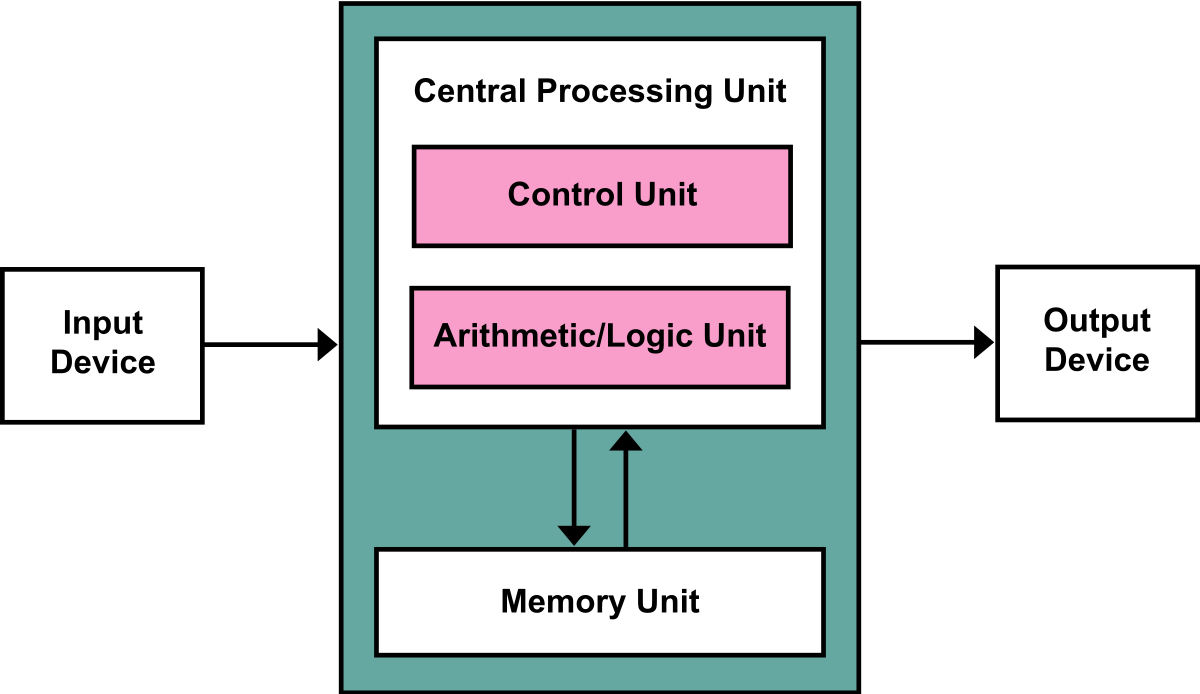
\includegraphics[width=0.7\textwidth]{figures/von_neumann.png}
\end{figure}
\begin{enumerate}[label=\alph*]
\item In 50 words or less, explain the role of the control unit. \\
\textbf{The control unit tells all other units what to do depending on the current state in control logic, which is determined by the current instruction. It holds the program counter and instruction register. }
\item In 50 words or less, explain the role of the ALU. \\
\textbf{The ALU performs all of the actual computation in a von Neumann machine. Data is loaded to and from memory, and processed through the ALU.}
\item For the LC-3 ISA, what does the control unit correspond to? \\
\textbf{The PC, IR, and control logic.}
\item For the LC-3 ISA, what are the inputs and outputs? \\
\textbf{Keyboard input and display (character display) output.}
\end{enumerate}

\newpage
\section*{LC-3 Assembly}
\subsection*{Problem 1}
\begin{figure}[!h]
    \centering
    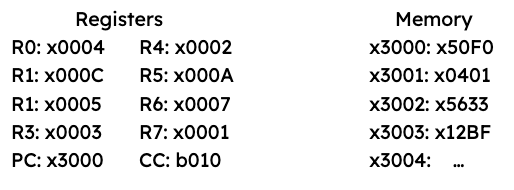
\includegraphics[width=1\textwidth]{figures/lc3_q1.png}
\end{figure}

\begin{figure}[!h]
    \centering
    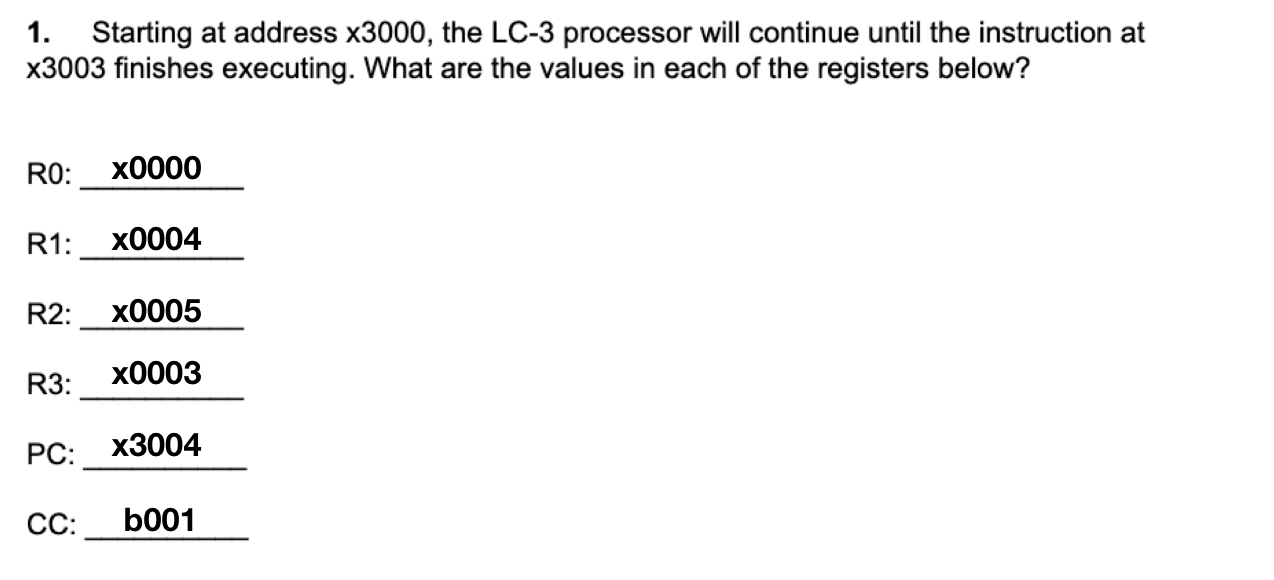
\includegraphics[width=1\textwidth]{figures/lc3_qsol1.jpg}
\end{figure}


\begin{figure}[!h]
    \centering
    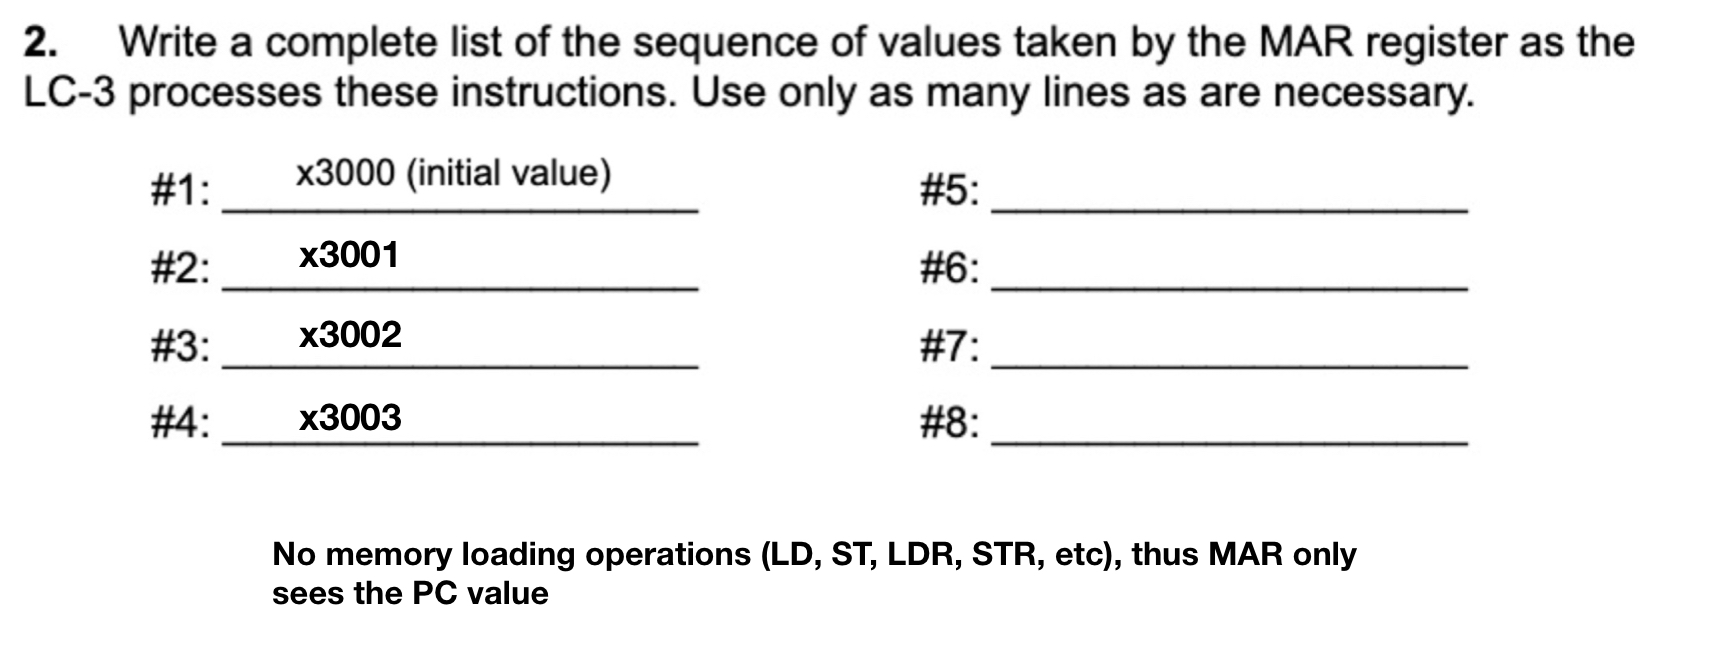
\includegraphics[width=1\textwidth]{figures/lc3_qsol2.jpg}
\end{figure}

\newpage
\subsection*{Problem 2}
Write an LC-3 Assembly program that compares two numbers in R2 and R3 and puts the larger number into R1. If the numbers are equal, then R1 is set equal  to 0. Use as many lines as necessary.

\begin{table}[!h]
\begin{tabular}{|l|l|l|}
\hline
\textbf{Location} & \textbf{Assembly} & \textbf{Comments}                             \\ \hline
x3000             & NOT R2, R2        & Set R2 to -R2 (step one)                      \\ \hline
x3001             & ADD R2, R2, \#1   & Set R2 to -R2 (step two)                      \\ \hline
x3002             & ADD R2, R3, R2    & Set R2 to R3 - R2                             \\ \hline
x3003             & BRn \#3           & If the result is negative, R2 \textgreater R3 \\ \hline
x3004             & BRp \#4           & If the result is positive, R3 \textgreater R2    \\ \hline
x3005             & AND R1, R1, \#0   & Else, set R1 to 0                             \\ \hline
x3006             & HALT              &                                               \\ \hline
x3007             & ADD R1, R2, \#0   & If R2 \textgreater R3, Set R1 to R2           \\ \hline
x3008             & HALT              &                                               \\ \hline
x3009             & ADD R1, R3, \#0   & If R3 \textgreater R2, Set R1 to R3           \\ \hline
x300A             & HALT              &                                               \\ \hline
\end{tabular}
\end{table}

\newpage
\subsection*{Problem 3}
Write two LC-3 Assembly programs that executes a bitwise OR operation and a bitwise XOR operation respectively on R4 and R5 and puts the result in R1. How might you extend these to support NOR and XNOR? \\
\textbf{OR} 
\begin{table}[!h]
\begin{tabular}{|l|l|l|}
\hline
\textbf{Location} & \textbf{Assembly} & \textbf{Comments}                   \\ \hline
x3000             & NOT R4, R4        & R4 \textless{}= $\sim$R4            \\ \hline
x3001             & NOT R5, R5        & R5 \textless{}= $\sim$R5            \\ \hline
x3002             & AND R1, R4, R5    & R1 \textless{}= R4'R5'              \\ \hline
x3003             & NOT R1, R1        & R1 \textless{}= (R4'R5')' = R4 + R5 \\ \hline
\end{tabular}
\end{table}
\\
\textbf{XOR}\\
\textbf{Remember that $p \bigoplus q = (p+q)(pq)'$}
\begin{table}[!h]
\begin{tabular}{|l|l|l|}
\hline
\textbf{Location} & \textbf{Assembly} & \textbf{Comments}                   \\ \hline
x3000             & AND R3, R4, R5    & R3 \textless{}= R4R5                \\ \hline
x3001             & NOT R4, R4        & R4 \textless{}= R4'                 \\ \hline
x3002             & NOT R5, R5        & R5 \textless{}= R5'                 \\ \hline
x3003             & AND R2, R4, R5    & R2 \textless{}= R4'R5'              \\ \hline
x3004             & NOT R2, R2        & R2 \textless{}= (R4'R5')' = R4 + R5 \\ \hline
x3005             & NOT R3, R3        & R3 \textless{}= (R4R5)'             \\ \hline
x3006             & AND R1, R2, R3    & R1 \textless{}= (R4 + R5)(R4R5)'    \\ \hline
\end{tabular}
\end{table}
\\
\textbf{NOR and XNOR would be adding an additional instruction NOT R1, R1 to negate the result.}

\newpage
\subsection*{Problem 4}
\begin{enumerate}[label=\alph*.]
\item Assuming LC-3 now has 32 registers, we want to increase the number of registers that we can specify in the LC-3 ADD instruction to 32. Is there a problem with this? Explain.
\\
\textbf{Yes, specifying 32 registers would require 5 bits per field, meaning 5 bits for SR1, 5 for SR2 and 5 for DR in the case of the 2 source version. This leaves only 1 bit for the opcode, which is not possible. If we were to extend the immediate version instead, we can fit the opcode, SR and DR into 14 bits, but this leaves only 2 bits for the immediate, which is extremely inconvenient at best.}

\item A memory's addressibility is 64 bits. What does that tell you about the size of the MAR and MDR, given a 64-bit ISA and $2^{20}$ memory locations?
\\
\textbf{64-bit addressibility means MDR must be 64 bits, as one address stores 64 bits of data. MAR can stay 20 bits as that is all that is needed to access one location.}

\item Say we have a memory consisting of 256 locations, and each location contains 16 bits. How many bits are required for the address for a byte-addressable system? Explain.
\\
\textbf{$256 = 2^8$, so 8 bits for the address. \\
        1 byte is 8 bits, $16/8 = $ 2 bits to offset into one location. \\
        So $8 + 2 = $ 10 bits are needed in total.}
\end{enumerate}

\end{document}
